\chapter{Results and Discussion}

\section{Classical MD simulations of intermediate A}
\subsection{Equilibration}
The equilibration process was assessed by monitoring different properties of the system during the last 5 ns equilibration run. The energy and density of the system were very stable with reasonable means and small standard deviations. Energy: $-1.695 \cdot 10^5 \, \pm \, 290 ~ \text{kcal/mol}$. Density: $1.046 \, \pm \, 0.001 ~ \text{g/cm}^3$. The structure of the system reached stability which can be seen from the small and stable RMSD of the protein's alpha carbon atoms in figure \ref{fig:A_equilibration}. The geometry of the active site was also stable with an average iron-iron distance of 6.2 Å (Fig.\,\ref{fig:A_equilibration}). The average membrane thickness was 37.0 Å (the phosphorus atom of phosphatidylcholine taken as reference) which is close to the experimentally reported thickness of 36.5 Å at 303 K for a pure POPC membrane \cite{kucerka2011}. The average area per lipid in the leaflet containing the narrower side of SCD1 was 63.2 Å$^2$ and 57.0 Å$^2$ in the leaflet containing the wider side of SCD1. The experimentally reported area per lipid for a pure POPC membrane at 303 K is 64.3 Å$^2$ \cite{kucerka2011} but deviations are expected when the membrane is perturbed by a transmembrane protein. Another membrane property easily calculated from MD simulations are the order parameters for the palmitoyl and oleoyl acyl chains of POPC \cite{Piggot2017}. Order parameters describe the conformation of the acyl chains and are a function of the angle between the C-H bond vector of each carbon atom in the chain and the membrane normal. Experimentally they are determined with NMR spectroscopy. The order parameters determined from the 5 ns equilibration run correspond well to the experimental values (Fig.\,\ref{fig:A_equilibration}). Again, some deviations from the values for a pure membrane are expected. Furthermore, accurate modelling of membrane properties was not the main goal of our study, so the results are considered satisfactory. 
\begin{figure}[htbp]
    \centering
    \begin{subfigure}{.49\textwidth}
        \centering
        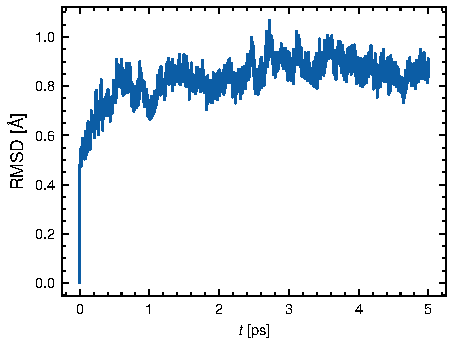
\includegraphics{Figures/A_rmsd.pdf}
    \end{subfigure}
    \begin{subfigure}{.49\textwidth}
        \centering
        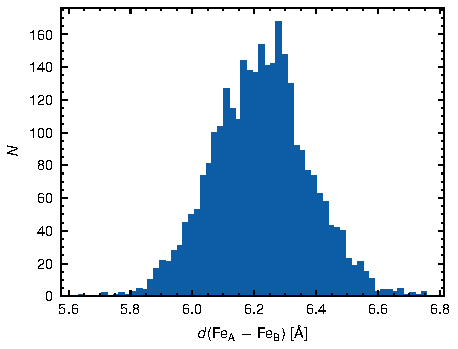
\includegraphics{Figures/A_fe-fe_hist.pdf}
    \end{subfigure}
    \par\bigskip
    \begin{subfigure}{.49\textwidth}
        \centering
        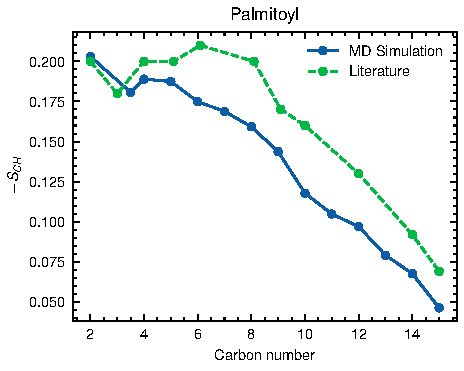
\includegraphics[width=\textwidth]{Figures/A_palmitoyl.pdf}
    \end{subfigure}
    \begin{subfigure}{.49\textwidth}
        \centering
        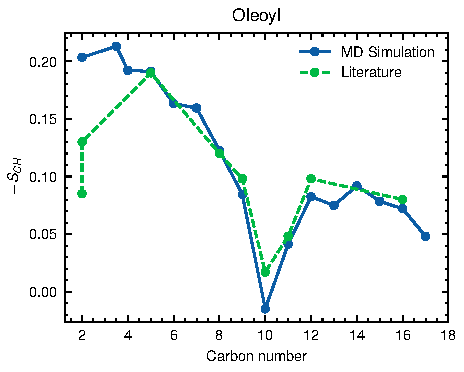
\includegraphics[width=\textwidth]{Figures/A_oleoyl.pdf}
    \end{subfigure}
    \caption{Data to assess the equilibration of intermediate A taken from the last 5 ns equilibration run. RMSD of the protein's backbone alpha carbon atoms with respect to the first frame (top left). Distribution of the iron-iron distance (top right). Average lipid order parameters for the palmitoyl chain of POPC (bottom left). Average lipid order parameters for the oleoyl chain of POPC (bottom right). Experimental values for the lipid order parameters are taken from \cite{Seelig1978,Perly1985}.}
    \label{fig:A_equilibration}
\end{figure}

\subsection{Production}
From experiments it is known that SCD1 specifically introduces a \textit{cis}-9 double bond and that the first hydrogen abstraction occurs at carbon nine of the acyl-CoA substrate \cite{Buist1996}. For this to happen the C$_8-$C$_9-$C$_{10}-$C$_{11}$ dihedral angle of the aliphatic chain should be in a negative \textit{gauche} conformation (-60$^{\circ}$) and the \textit{pro}-R (H$_{9}$) hydrogen on carbon nine should be relatively close to the oxo group (O$_{\text{B}}$) on Fe$_{\text{B}}$ of intermediate A.

Based on the three 500 ns production runs of intermediate A it was concluded that the aliphatic chain of ST9 was not in a favorable orientation for the reaction to occur (Fig.\,\ref{fig:A_prodcution}). In both runs one and three the O$_{\text{B}}-$H$_9$ distance quickly increased to around 4.5 Å and rarely dropped below 4 Å which is presumably too far away for initiating the reaction. In the second run the O$_{\text{B}}-$H$_9$ distance readily dropped below 3 Å for 400 ns, but the C$_8-$C$_9-$C$_{10}-$C$_{11}$ dihedral angle adopted predominantly angles typical of the unfavorable \textit{anti} ($\pm180^{\circ}$) conformation. On top of that, the O$_{\text{B}}-$H$_9$ distance increased to around 4 Å in the last 100 ns of the simulation.

Compared to the crystal structure of SCD1 \cite{Bai2015} (Fig.\,\ref{fig:Crystal_water}) the Asn261 side chain rotates already during the equilibration, so that the amide nitrogen forms a H-bond with the structural water molecule above it. This rotation is not surprising and was discussed in section 1.3.1. The problem now is that nothing is stabilizing the axial oxo group on Fe$_{\text{B}}$ or the amide oxygen of Asn261. In all three production runs an entrance of a solvent water molecule from the substrate tunnel into the active site was observed (Fig.\,\ref{fig:A_prodcution}) which stabilizes the side chain of Asn261 by forming a H-bond with it (Fig.\,\ref{fig:intA_run1}). To accommodate the solvent water molecule the aliphatic chain needs to move slightly away from the active site which explains the increase in the O$_{\text{B}}-$H$_9$ distance in all three production runs. In the second production run the Asn261 residue adopts a slightly different conformation where the side chain amide nitrogen forms an H-bond with a backbone carbonyl oxygen of His167 (Fig.\,\ref{fig:intA_run2}). The different conformation of Asn261 possibly explains the preference for the \textit{anti} conformation of the C$_8-$C$_9-$C$_{10}-$C$_{11}$ dihedral angle in the second production run.

\begin{figure}[htbp]
    \centering
    \begin{subfigure}{\textwidth}
        \centering
        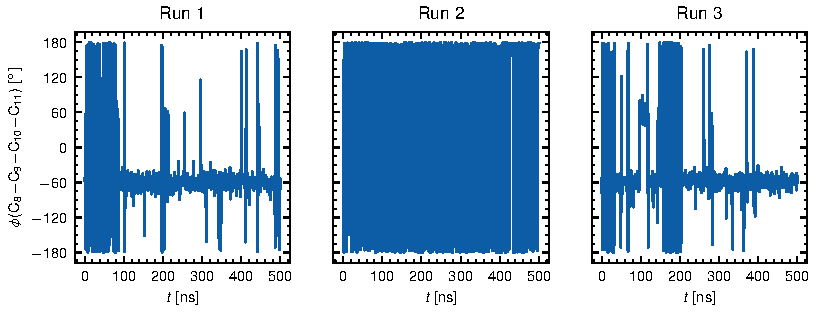
\includegraphics[width=\textwidth]{Figures/A_C9-C10_all.pdf}
    \end{subfigure}
    \par\bigskip
    \begin{subfigure}{\textwidth}
        \centering
        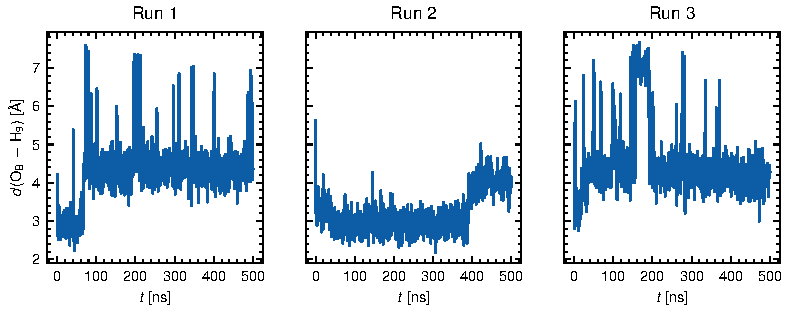
\includegraphics[width=\textwidth]{Figures/A_Ob-H9_all.pdf}
    \end{subfigure}
    \par\bigskip
    \begin{subfigure}{\textwidth}
        \centering
        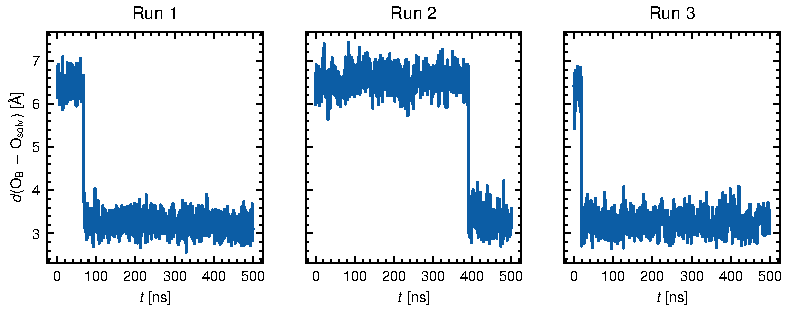
\includegraphics[width=\textwidth]{Figures/A_Ob-Ow_all.pdf}
    \end{subfigure}
    \caption{Data from the three 500 ns production runs of intermediate A: value of the C$_8-$C$_9-$C$_{10}-$C$_{11}$ dihedral angle of the substrate (top); distance between the oxo oxygen (O$_{\text{B}}$) and \textit{pro}-R hydrogen on C$_9$ (H$_{9}$) that needs to get abstracted (middle); distance between the oxo oxygen (O$_{\text{B}}$) and oxygen of a nearby solvent water molecule in the substrate tunnel (bottom). Note: due to the cyclical nature of the dihedral angles the values around 180$^{\circ}$ and $-$180$^{\circ}$ correspond to the same \textit{anti} conformation.}
    \label{fig:A_prodcution}
\end{figure}

\begin{figure}[!htb]
    \centering
    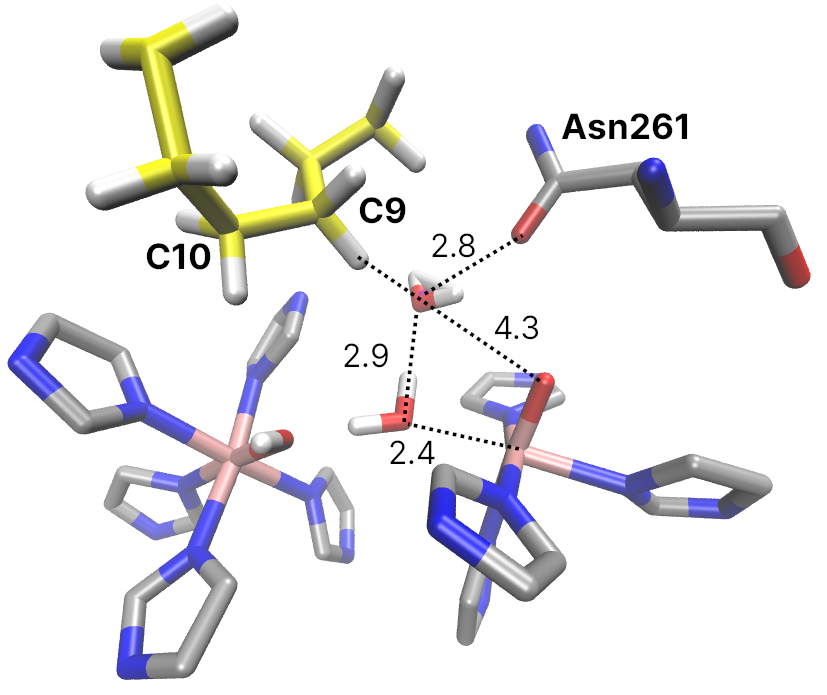
\includegraphics[width=0.7\textwidth]{Figures/int_A_run1.png}
    \caption{Structure of the active site after the entrance of a solvent water molecule during MD simulations of intermediate A. Residues are shown as sticks. Distances are shown in Å. Colours: silver, protein carbons; red, oxygen; blue, nitrogen; white, hydrogen; yellow, carbons of stearoyl-CoA; pink, iron. Protein hydrogen atoms are left out for clarity.}
    \label{fig:intA_run1}
\end{figure}

\subsection{Proposing a new intermediate}
MD simulations suggest that intermediate A is not able to form a reactive complex with the substrate that would be consistent with the experimentally determined selectivity of SCD1. Additionally, Asn261 seems to have an important role in controlling the positioning and conformation of the substrate. Asn261 was not included in the original cluster model study which proposed intermediate A \cite{Yu2019}. Furthermore, Asn261 is conserved among transmembrane desaturases from different organisms \cite{Bai2015}, so it is reasonable to assume it serves some function. To the best of our knowledge the function of Asn261 has not been previously discussed or investigated with mutagenesis studies. Based on these findings we propose a new intermediate B where the water and oxo ligands on Fe$_{\text{B}}$ exchange places (Fig.\,\ref{fig:IntA_IntB}). This would enable formation of an H-bond between the water ligand and the amide oxygen of the Asn261 side chain. The formation of intermediate B should be possible from the same species (Int3$_{\text{A}-\alpha}$) that leads to the formation of intermediate A in the proposed mechanism (Fig.\,\ref{fig:SCD1_mechanism}). Intermediate B was not discussed in the cluster model study possibly because no TS leading to it was found, but the study did not consider the possible participation of an explicit solvent water molecule. It is known that the barrier for rearrangement of a dihydroxoiron(IV) complex, like Int3$_{\text{A}-\alpha}$, to an iron(IV)-oxo species (intermediate A/B) is reduced by participation of an explicit solvent water molecule \cite{Petit2014}. Our MD simulations showed that solvent water molecules from the substrate tunnel can enter the active site, so the formation of intermediate B should be possible.

\section{Classical MD simulations of intermediate B}
\subsection{Equilibration}
The analysis of the equilibration was performed in the same way as for intermediate A. Energy and density of the system were very stable with reasonable means and small standard deviations. Energy: $-1.695 \cdot 10^5 \, \pm \, 290 ~ \text{kcal/mol}$. Density: $1.046 \, \pm \, 0.001 ~ \text{g/cm}^3$. The structure of the system reached stability which can be seen from the small and stable RMSD of protein's alpha carbon atoms in figure \ref{fig:B_equilibration}. The geometry of the active site was also stable with an average iron-iron distance of 5.64 Å (Fig. \ref{fig:B_equilibration}). The slight reduction in the iron-iron distance is due to the formation of a short H-bond between the oxo group on Fe$_{\text{B}}$ and the hydroxide group on Fe$_{\text{A}}$. The average membrane thickness was 37.0 Å (the phosphorus atom of phosphatidylcholine taken as reference) which is close to the experimentally reported thickness of 36.5 Å at 303 K for a pure POPC membrane \cite{kucerka2011}. The average areas per lipid are 65.0 Å$^2$ and 59.1 Å$^2$, similar as for intermediate A. The order parameters determined from the 5 ns equilibration run correspond well to the experimental values (Fig.\,\ref{fig:B_equilibration}).

\subsection{Production}
In all three 1 $\mu$s production runs of intermediate B a favourable reactive complex with the substrate was formed (Fig.\,\ref{fig:B_production}). The O$_{\text{B}}-$H$_9$ distance was on average 3.4 Å and readily dropped below 3 Å with a minimum distance of 2.3 Å. The C$_8-$C$_9-$C$_{10}-$C$_{11}$ dihedral angle adopted predominantly angles typical for the favourable negative \textit{gauche} conformation ($-60^{\circ}$). Time series of the values are shown in figure \ref{fig:B_appendix} in the appendix. A solvent water molecule would occasionally enter the active site but also quickly exit. As expected, the active site water ligand maintained a constant H-bond (2.7 Å on average) with the amide oxygen of the Asn261 side chain but also an additional H-bond (2.8 Å on average) with the backbone oxygen of Val260 (Fig.\,\ref{fig:intB_run1}). The additional H-bonds combined with the substrate orientation suggest that intermediate B is a more favourable reactive intermediate than the previously suggested intermediate A.

\begin{figure}[htbp]
    \centering
    \begin{subfigure}{.49\textwidth}
        \centering
        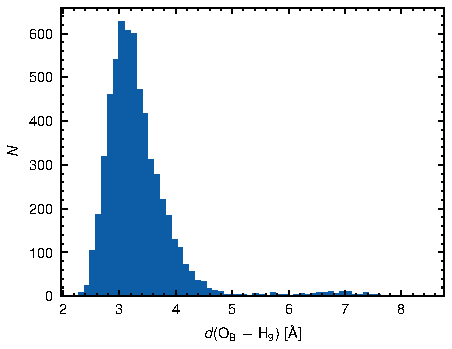
\includegraphics{Figures/B_Ob-H9_hist.pdf}
    \end{subfigure}
    \begin{subfigure}{.49\textwidth}
        \centering
        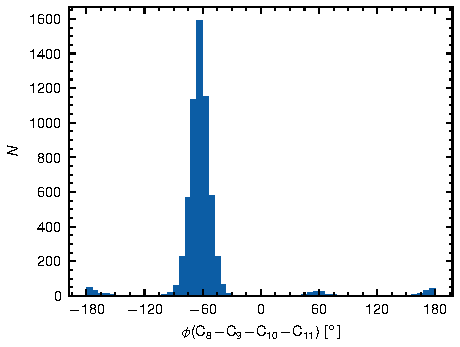
\includegraphics{Figures/B_C9-C10_hist.pdf}
    \end{subfigure}
    \caption{Distribution of the distance between the oxo oxygen (O$_{\text{B}}$) and the \textit{pro}-R hydrogen on C$_{9}$ (H$_{9}$) that needs to get abstracted during the three 1 $\mu$s production runs of intermediate B (left). Distribution of the substrate's C$_8-$C$_9-$C$_{10}-$C$_{11}$ dihedral angle during the three 1 $\mu$s production runs of intermediate B (right).}
    \label{fig:B_production}
\end{figure}
\begin{figure}[!htb]
    \centering
    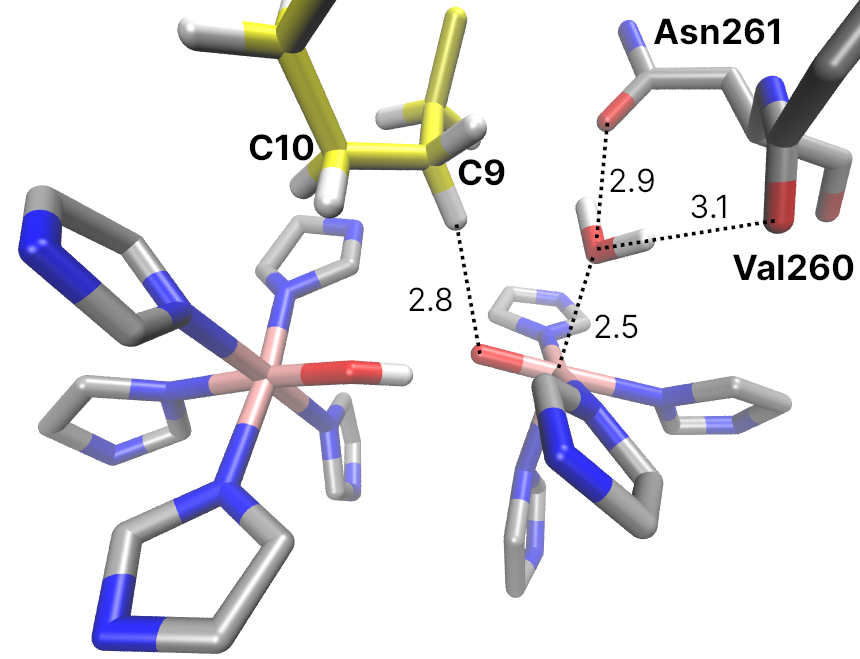
\includegraphics[width=0.7\textwidth]{Figures/int_B_run1.png}
    \caption{Structure of the active site during MD simulations of intermediate B. Residues are shown as sticks. Distances are shown in Å. Colours: silver, protein carbons; red, oxygen; blue, nitrogen; white, hydrogen; yellow, carbons of stearoyl-CoA; pink, iron. Protein hydrogen atoms are left out for clarity.}
    \label{fig:intB_run1}
\end{figure}

\section{GFN2-xTB cluster model}
Even though we showed that intermediate B is potentially a more favourable reactive intermediate, intermediate A was chosen for evaluating the applicability of the GFN2-xTB method, so that the results can be compared to the B3LYP cluster model study \cite{Yu2019}. Optimization of the reported structure of intermediate A with GFN2-xTB resulted only in slight changes where C$_9$ and C$_{10}$ move away from the active site by 0.74 Å and 0.48 Å (Tab.\,\ref{tab:xtb_geoemtry}). The relaxed PES scan along the O$_{\text{B}}-$H$_9$ distance predicts an energy barrier of 7.0 kcal/mol (Fig.\,\ref{fig:xtb_cluster}). This is quite close to the reported barrier of 10.0 kcal/mol. The structure of the TS is also close to the reported structure (Tab.\,\ref{tab:xtb_geoemtry}). The O$_{\text{B}}-$H$_9$ distance is predicted to be 0.15 Å longer and the C$_{\text{9}}-$H$_{\text{9}}$ distance 0.06 Å shorter. The spin densities of the TS correspond well to the reported values (Tab.\,\ref{tab:xtb_spin}). The biggest difference is in the distribution of spin between Fe$_{\text{B}}$ and O$_{\text{B}}$ where GFN2-xTB predicts a higher radical character of O$_{\text{B}}$. The reaction is predicted to be exothermic with a reaction energy of -7.1 kcal/mol while in the B3LYP cluster study the reaction is predicted to be endothermic with a reaction energy of 5.9 kcal/mol. GFN2-xTB clearly overstabilizes the energy of the final state corresponding to Int5$_{\text{A}-\alpha}$ in figure~\ref{fig:Desaturation}.

\begin{figure}[htbp]
    \centering
    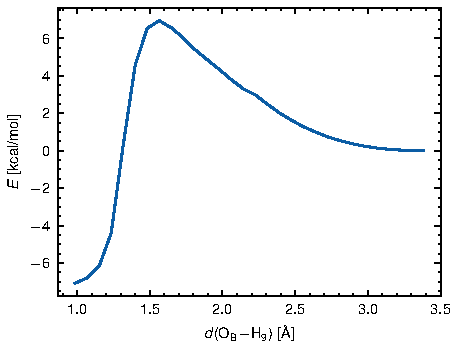
\includegraphics[width=0.6\textwidth]{Figures/xtb_cluster.pdf}
    \caption{Relaxed potential energy surface along the O$_{\text{B}}-$H$_9$ distance obtained with GFN2-xTB for a cluster model of intermediate A. The predicted energy barrier is 7.0 kcal/mol. The starting state is on the right.}
    \label{fig:xtb_cluster}
\end{figure}

\begin{table}[htbp]
\caption{Geometric properties of intermediate A and the TS predicted by the GFN2-xTB cluster model relaxed potential energy surface scan of intermediate A. Predicted values with B3LYP are taken from \cite{Yu2019}. Complete structures are shown in figures~\ref{fig:xtb_TS} and \ref{fig:xtb_intA}.}
\centering
\begin{tabular}{@{}ccccc@{}}
\cmidrule(l){2-5}
                                               & \multicolumn{2}{c}{\textbf{Intermediate A}} & \multicolumn{2}{c}{\textbf{TS}}    \\ \midrule
\textbf{Property}                              & \textbf{B3LYP}      & \textbf{GFN2-xTB}     & \textbf{B3LYP} & \textbf{GFN2-xTB} \\ \midrule
$d($Fe$_{\text{A}}-$Fe$_{\text{B}})$           & 6.03 Å              & 6.31 Å                & 5.90 Å         & 5.93 Å            \\
$d($Fe$_{\text{B}}-$O$_{\text{W}})$            & 2.23 Å              & 2.42 Å                & 2.16 Å         & 2.36 Å            \\
$d($Fe$_{\text{B}}-$O$_{\text{B}})$            & 1.62 Å              & 1.63 Å                & 1.72 Å         & 1.68 Å            \\
$d($O$_{\text{B}}-$H$_{\text{9}})$             & 2.63 Å              & 3.38 Å                & 1.42 Å         & 1.57 Å            \\
$d($C$_{\text{9}}-$H$_{\text{9}})$             & 1.10 Å              & 1.09 Å                & 1.23 Å         & 1.17 Å            \\
$d($O$_{\text{B}}-$C$_{\text{9}})$             & 3.72 Å              & 4.45 Å                & 2.64 Å         & 2.73 Å            \\
$d($Fe$_{\text{A}}-$O$_{\text{A}})$            & 1.92 Å              & 2.12 Å                & 1.92 Å         & 2.12 Å            \\
$d($O$_{\text{A}}-$C$_{\text{10}})$            & 3.41 Å              & 3.89 Å                & 3.44 Å         & 4.28 Å            \\
$\alpha$(Fe$_{\text{B}}-$O$_{\text{B}}-$H$_9$) & 143$^{\circ}$       & 135$^{\circ}$         & 165$^{\circ}$  & 162$^{\circ}$     \\ \bottomrule
\end{tabular}
\label{tab:xtb_geoemtry}
\end{table}

GFN2-xTB performed surprisingly well in modelling the HAA step by intermediate A, especially in predicting the geometries. Both the geometries and the reaction barrier are close to  B3LYP results. A big error is made in the reaction energy but our focus is on the reaction barrier and the plan in the end is to correct energies with higher level of theory single point calculations, so the good geometry predictions are promising.


\section{Studying the reactivity of intermediate B} 
\subsection{Classical MD simulations with the TIP3P water model}
The equilibration procedure was analyzed in the same way as with the OPC water model (Fig.\,\ref{fig:TIP3P_equilibration}). Energy and density fluctuations were very small. The RMSD of alpha carbon atoms was small and stable. The lipid order parameters and other membrane properties were similar as before: thickness 37.3 Å; areas per lipid 62.7 and 55.7 Å$^2$. The substrate was again in a favorable reactive orientation during the 500 ns production run with the C$_8-$C$_9-$C$_{10}-$C$_{11}$ dihedral angle predominantly being around $-60^{\circ}$ and the O$_{\text{B}}-$H$_{\text{9}}$ distance around 3.2 Å and readily dropping below 3 Å (Fig.\,\ref{fig:TIP3P_production}). These simulations were performed as a prerequisite for QM/MM MD simulations with GFN2-xTB because the interface between Amber and external QM software does not support the OPC water model, but the results still provide support for the favourable properties of intermediate B. 

\begin{figure}[htbp]
    \centering
    \begin{subfigure}{.49\textwidth}
        \centering
        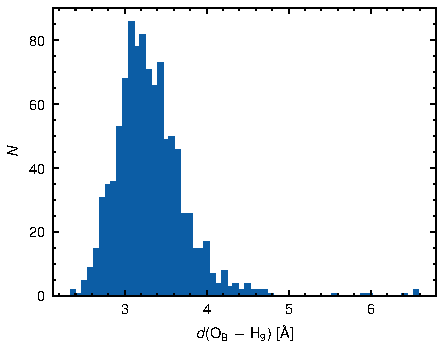
\includegraphics{Figures/TIP3P_Ob-H9_hist.pdf}
    \end{subfigure}
    \begin{subfigure}{.49\textwidth}
        \centering
        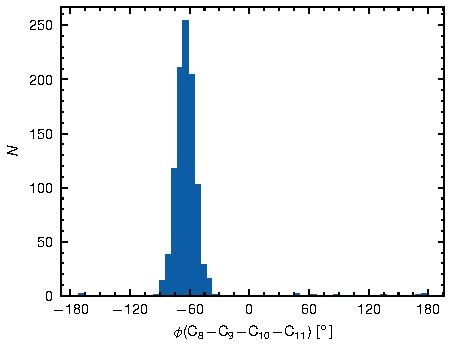
\includegraphics{Figures/TIP3P_C9-C10_hist.pdf}
    \end{subfigure}
    \caption{Distribution of the distance between the oxo oxygen (O$_{\text{B}}$) and the \textit{pro}-R hydrogen on C$_{9}$ (H$_{9}$) that needs to get abstracted during the 500 ns production run of intermediate B (left) with the TIP3P water model. Distribution of the substrate's C$_8-$C$_9-$C$_{10}-$C$_{11}$ dihedral angle during the 500 ns production run of intermediate B (right).}
    \label{fig:TIP3P_production}
\end{figure}

\subsection{GFN2-xTB QM/MM MD simulations}
In the first and third 500 ps production runs with GFN2-xTB no major structural changes in the active site occurred which implies that the previously developed force field parameters were of good quality. The average iron-iron distance differs only by 0.05 Å from the average distance in the classical MD simulations with the TIP3P water model. The substrate was again in a favourable reactive orientation (Fig.\,\ref{fig:xtb_production}). The O$_{\text{B}}-$H$_{\text{9}}$ was even shorter on average by 0.12 Å with a minimal distance below 2 Å. The active site water ligand maintained a constant H-bond with the side chain of Asn261 and the backbone oxygen of Val260. These results further support the favourable nature of intermediate B, but problems occurred in the second production run where the hydroxide on Fe\textsubscript{A} spontaneously abstracted the \textit{pro}-S hydrogen on C$_{10}$ (Fig.\,\ref{fig:xtb_appendix}). After the abstraction the substrate was in an unfavourable orientation for the second HAA. This indicates that GFN2-xTB does not provide a perfect description of the system which is not surprising when simulating dynamics of a system as complicated as this. Still, the two successful 500 ps runs where the system behaved reasonably are promising.
\begin{figure}[htbp]
    \centering
    \begin{subfigure}{.49\textwidth}
        \centering
        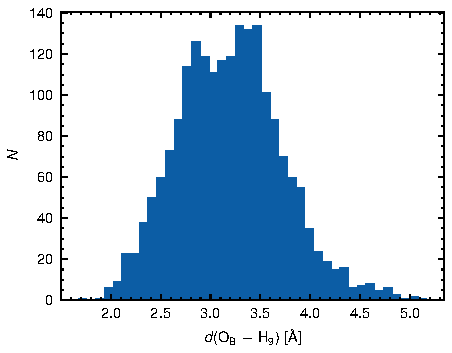
\includegraphics{Figures/xtb_Ob-H9_hist.pdf}
    \end{subfigure}
    \begin{subfigure}{.49\textwidth}
        \centering
        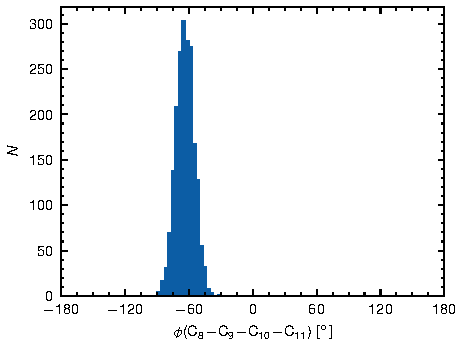
\includegraphics{Figures/xtb_C9-C10_hist.pdf}
    \end{subfigure}
    \caption{Distribution of the distance between the oxo oxygen (O$_{\text{B}}$) and the \textit{pro}-R hydrogen on C$_{9}$ (H$_{9}$) that needs to get abstracted during the first and third 500 ps production runs of intermediate B with GFN2-xTB (left). Distribution of the substrate's C$_8-$C$_9-$C$_{10}-$C$_{11}$ dihedral angle during the first and third 500 ps production runs of intermediate B with GFN2-xTB (right).}
    \label{fig:xtb_production}
\end{figure}

\subsection{GFN2-xTB PES scan}
In the starting structure selected for the PES scan with GFN2-xTB the O$_{\text{B}}-$H$_{\text{9}}$ distance was 3.22 Å and the Fe$_{\text{B}}-$O$_{\text{B}}-$H$_{\text{9}}$ angle was 105$^{\circ}$. The PESs predicted for both the periodic (with PBCs) and non-periodic system are shown in figure \ref{fig:PES_xtb}. Only the total energy of the QM region together with QM-MM interactions is plotted because the energy of the MM region usually introduces a lot of noise due to its size. In the case of the periodic system, unreasonably large energy fluctuation between structures on the PES are predicted even though the structures are reasonable and stable from one step to the next. This probably occurs because of the use of a finite cutoff of 20 Å for electrostatic QM-MM interactions. Electrostatic interactions are very long-range and using a simple cutoff will always lead to discontinuities in the energy, especially if the QM region has a large charge of +4 like here. Because of this it was necessary to perform the PES scan for a non-periodic system where all MM point charges are included in the QM Hamiltonian. This resulted in a more reasonable PES with a predicted barrier of 11.4 kcal/mol (Fig.\,\ref{fig:PES_xtb}). The structure of the TS is reasonable and is shown in figure \ref{fig:xtb_scan_ts}.

\begin{figure}[htbp]
    \centering
    \begin{subfigure}{.49\textwidth}
        \centering
        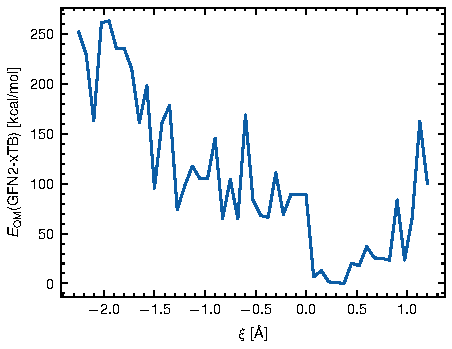
\includegraphics{Figures/PES_xtb_PBC.pdf}
    \end{subfigure}
    \begin{subfigure}{.49\textwidth}
        \centering
        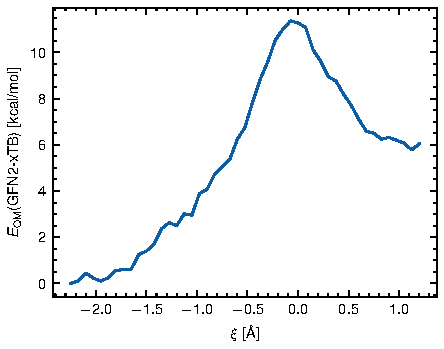
\includegraphics{Figures/PES_xtb.pdf}
    \end{subfigure}
    \caption{Potential energy surfaces obtained from a relaxed scan with GFN2-xTB for intermediate B along the reaction coordinate $\xi$ with (left) and without (right) periodic boundary conditions. Only the total energy of the QM region together with QM-MM interactions is plotted because the energy of the MM region usually introduces a lot of noise due to its size.}
    \label{fig:PES_xtb}
\end{figure}
\begin{figure}[htbp]
    \centering
    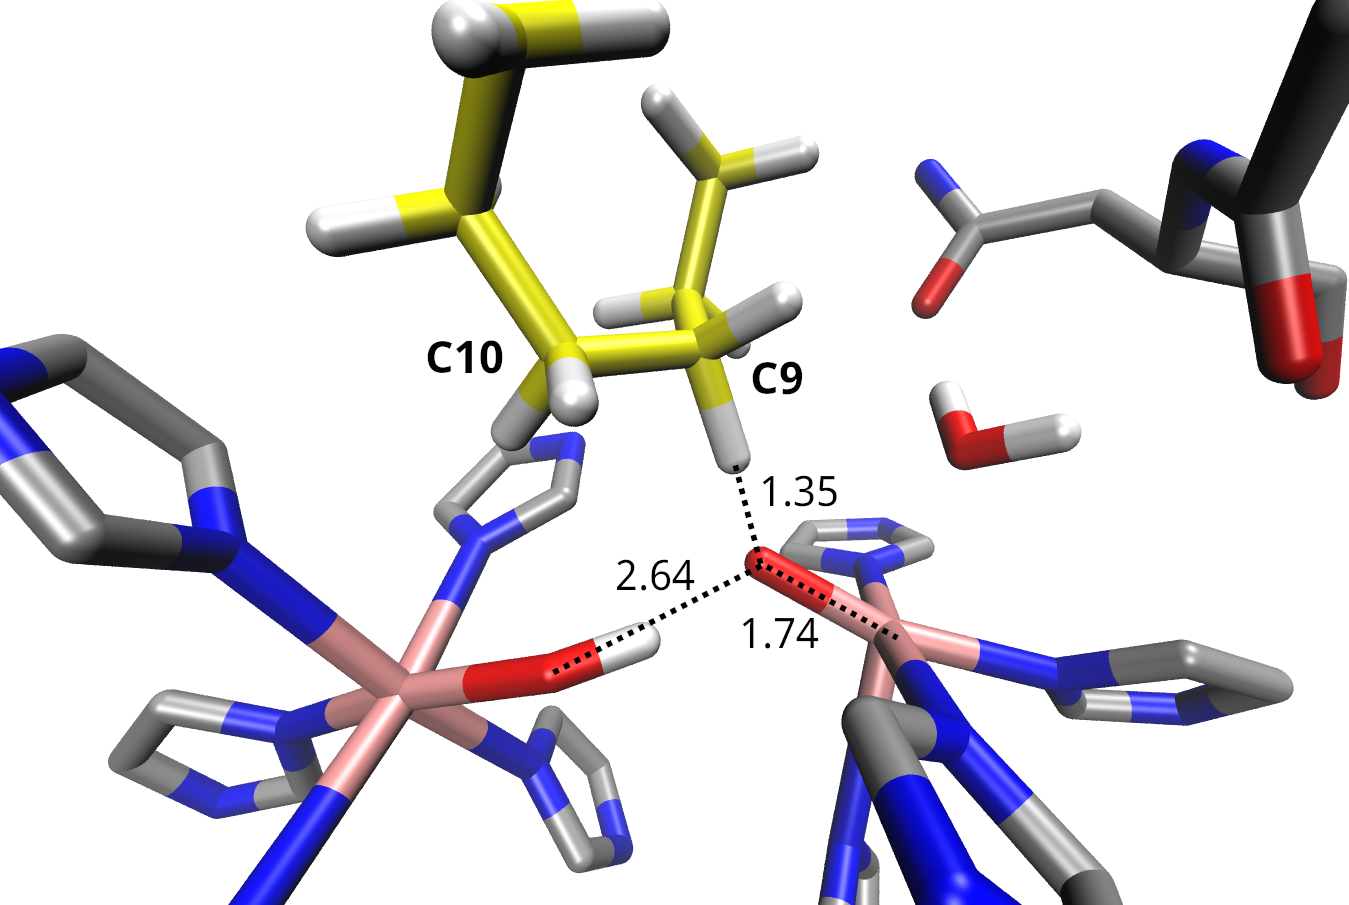
\includegraphics[width=0.8\textwidth]{Figures/new_scan_ts.png}
    \caption{Structure of the TS predicted from a relaxed PES scan with GFN2-xTB of intermediate B along the reaction coordinate $\xi$. Residues are shown as sticks. Distances are shown in Å. Colours: silver, protein carbons; red, oxygen; blue, nitrogen; white, hydrogen; yellow, carbons of stearoyl-CoA; pink, iron. Protein hydrogen atoms are left out for clarity.}
    \label{fig:xtb_scan_ts}
\end{figure}

\subsection{B3LYP single-point calculations}
Single point energies of all structures on the GFN2-xTB PES for the non-periodic system were recalculated with B3LYP (Fig.\,\ref{fig:b3lyp_spc}). The large spike in energy at higher values of the reaction coordinate occurs because of convergence problems which is not uncommon for complicated transition metal systems. The problem was not investigated in great detail because we are mostly interested in the reaction barrier and no problems occurred for neighbouring structures, so it appears that this point of discontinuity can most likely be ignored. The barrier is increased by 8.5 kcal/mol to 19.9 kcal/mol. This is on the higher end for most enzymes. As a reference, numerous enzymatic reactions exibit a rate constant of 10$^3$ s$^{-1}$, which, according to the Eyring equation, corresponds to a free energy barrier of 13.4 kcal/mol. Technically we are comparing free energy differences to differences in static DFT energies, but they usually do not differ too much because entropic contributions tend to be small \cite{Claeyssens2006}. It is important to note that only one pathway obtained with GFN2-xTB was considered, so there are many ways to improve this estimate.
\begin{figure}[htbp]
    \centering
    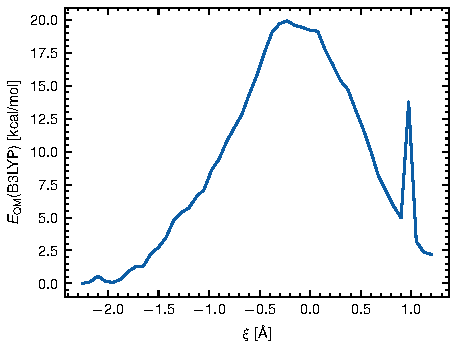
\includegraphics[width=0.6\textwidth]{Figures/PES_b3lyp.pdf}
    \caption{Single point energies calculated with B3LYP(15\% exact exchange)/def2tzvp with Grimme D3 disperssion of each structure from the PES scan with GFN2-xTB of intermediate B along the reaction coordinate $\xi$.}
    \label{fig:b3lyp_spc}
\end{figure}

\subsection{Potential of mean force}
Umbrella sampling was used to predict the free energy barrier of the first HAA step by intermediate B with GFN2-xTB. Even though large energy fluctuations occurred in the PES scan when using PBCs, molecular dynamics in each umbrella sampling window was performed with PBCs. This assumes that the finite cutoff for electrostatic QM-MM interactions does not affect the distribution along the reaction coordinate and in turn the PMF. It was tried to perform umbrella sampling for the non-periodic system but this always resulted in nonphysical outcomes where some atoms from the QM region moved far away from the system. During umbrella sampling it was also necessary to restrain the C$-$H bonds on C$_{10}$ because otherwise the hydroxide on Fe\textsubscript{A} would spontaneously abstract a hydrogen from C$_{10}$ in some umbrella sampling windows. This is similar to what happened in the second QM/MM MD production run and again shows some limitations of GFN2-xTB. 

The distribution of the reaction coordinate in each umbrella sampling window after constraining the C$-$H bonds on C$_{10}$ is shown in figure \ref{fig:umbrella_histograms}. There is good overlap between neighbouring histograms and the corresponding PMF computed using the WHAM method is shown in figure \ref{PMF}. Problems occurred in the umbrella sampling window at $\xi = -0.225$ Å where O\textsubscript{B} adopts an axial position on Fe\textsubscript{B} by displacing the water ligand (Fig.\,\ref{fig:pmf_window_28}). This is probably unreasonable but it only occurred in one window, so it should not drastically affect the PMF, especially when there is good overlap between histograms. Interestingly, GFN2-xTB predicts a hydrogen atom transfer from O\textsubscript{A} to O\textsubscript{B} after the TS which results in a water ligand on Fe\textsubscript{B} and an oxo group on Fe\textsubscript{A}. This is not unreasonable but we cannot be sure if it is only an artefact of using GFN2-xTB. The predicted free energy barrier is 8.4 kcal/mol. We know from the PES scans that GFN2-xTB underestimates the potential energy barrier by 8.5 kcal/mol compared to B3LYP. Assuming that all the correction is in the potential energy means that our best estimate of the free energy barrier is $8.4 + 8.5 = 16.9$ kcal/mol, a certainly reachable value. Our estimate is not without flaws but it suggests that intermediate B has favourable reactive properties on top of the favourable dynamical properties determined by classical MD simulations.
\begin{figure}[ht]
    \centering
    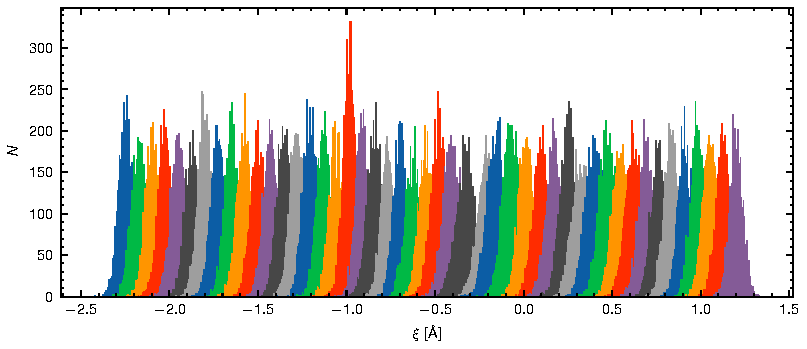
\includegraphics[width=\textwidth]{Figures/umbrella_histograms.pdf}
    \caption{Distribution of the reaction coordinate $\xi$ of intermediate B during molecular dynamics simulations in each biased umbrella sampling window.}
    \label{fig:umbrella_histograms}
\end{figure}
\begin{figure}[htbp]
    \centering
    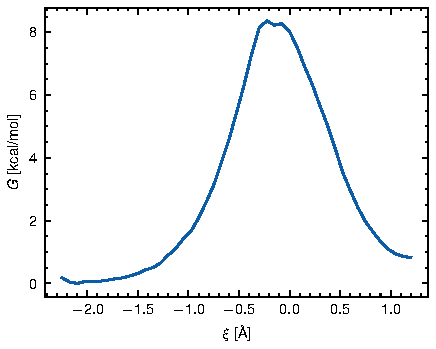
\includegraphics[width=0.6\textwidth]{Figures/PMF.pdf}
    \caption{Potential of mean force for the first HAA step by intermediate B computed with WHAM from biased umbrella sampling windows along the reaction coordinate $\xi$.}
    \label{fig:PMF}
\end{figure}